\chapter{Accelerazione del Metodo delle Potenze: Metodo di Chebyshev}

Supponiamo che, dopo $n^*$ iterazioni con il metodo delle potenze, la stima $k^*$ dell'autovalore fondamentale sia considerata adeguata e non venga più aggiornata. Tuttavia, l'autovettore fondamentale potrebbe non essere ancora sufficientemente accurato. Per migliorarlo, si può continuare a iterare.
Il metodo delle potenze procederebbe come segue:

\[\begin{aligned}
\phi^{(n^* + 1)}\ &=\ \frac{1}{k^*} \mathbf{K} \phi^{(n^*)}\ \ ,\\
\phi^{(n^* + 2)}\ &=\ \frac{1}{k^*} \mathbf{K}\ =\ \phi^{(n^* + 1)}\ =\ \left(\frac{1}{k^*} \mathbf{K}\right)^{2} \phi^{(n^*)}\ \ ,\\
&\vdots\\
\phi^{(n^* + n)}\ &=\ \left(\frac{1}{k^*} \mathbf{K}\right)^{n} \phi^{(n^*)}\ \ .
\end{aligned}\]



In questo processo, il vettore $\phi^{(n^*)}$ è una sorta di nuovo vettore iniziale a cui vengono applicate le successive potenze della matrice $\frac{1}{k^*}\mathbf{K}$.

%
%
\section{Polinomi Matriciali e Accelerazione}

L'autovalore fondamentale di $\mathbf{K}/k^*$  è  $\frac{k_1}{k^*} \approx 1$. Se, al posto della singola matrice $\left(\frac{1}{k^*}\mathbf{K}\right)^n$, si utilizza un polinomio matriciale di ordine n, $P_n\left(\mathbf{K}/k^*\right)$, si può ottenere una convergenza più rapida attraverso una scelta appropriata dei coefficienti del polinomio.

Il processo per $\phi^{(n^* + n)}$ viene sostituito da:
\[\phi^{(n^* + n)}\ =\ P_{n} \left(\frac{\mathbf{K}}{k^*}\right) \phi^{(n^*)}\ \ .\]

Espandendo il vettore $\phi^{(n^*)}$ in termini degli autovettori della matrice $\mathbf{K}$:

\[\phi^{(n^*)} = c_{1} \varphi_{1} + \sum_{h \geq 2} c_{h} \varphi_{h}\ \ .\]


%
%
\subsection{Applicazione dei Polinomi di Chebyshev}

Si può scrivere:

\[\phi^{(n^* + n)}\ =\ P_n \left(\frac{\mathbf{K}}{k^*}\right) \left[ c_1 \varphi_1 + \sum_{h \geq 2} c_h \varphi_h \right]\ =\ c_1 P_n \left(\frac{k_1}{k^*}\right) \varphi_1 + \sum_{h \geq 2} c_h P_n \left(\frac{k_h}{k^*}\right) \varphi_h\ \ .\]


Dati tutti gli autovalori $k_h$ ($h \geq 2$) di $\mathbf{K}$, scegliendo un ordine n sufficientemente alto del polinomio matriciale, si possono determinare i suoi coefficienti in modo che:

\[P_n \left(\frac{k_1}{k^*}\right)\ \approx\ P_n(1)\ =\ 1;\ \qquad	
\ P_n \left(\frac{k_h}{k^*}\right) = 0 \quad \forall h \geq 2\ \ .\]

Così l'equazione per $\phi^{(n^* + n)}$ si ridurrebbe a:

\[\phi^{(n^* + n)}\ =\ c_1 \varphi_1\ \ .\]

In altre parole, con un numero finito di interazioni (un numero finito di potenze $\mathbf K / k^*$) raggiungeremmo la soluzione esatta.

Tuttavia, poiché la conoscenza di tutti gli autovalori di $\mathbf{K}$ è impraticabile, invece di cercare di annullare la somma

\[\sum_{h \geq 2} c_h P_n \left(\frac{k_h}{k^*}\right) \varphi_h\ \ ,\]

è meglio minimizzarla.

%
%
\subsection{Minimizzazione del Residuo}

Data una stima del dominance ratio $\sigma$ e assumendo che tutti gli autovalori per $h \geq 2$ siano comunque non negativi, si ha:

\[0 \leq \frac{k_h}{k^*} \leq \sigma < 1 \qquad \forall\ h \geq 2\ \ .\]

Il problema di minimizzazione da risolvere è:

\[P_n(1)\ =\ 1;\ \qquad \min_{a_0, a_1, \dots, a_n}\, \max_{0 \leq x \leq \sigma}\, |P_n(x)|\ \ .\]

La soluzione a questo problema è data dai seguenti polinomi:

\[P_n(x) = \frac{C_n\left(\frac{2x}{\sigma} - 1\right)}{C_n\left(\frac{2}{\sigma} - 1\right)}\ \ ,\]

dove $C_n$ sono i polinomi di Chebyshev, definiti dalla relazione di ricorrenza:
$C_0(t) = 1$ , 
$C_1(t) = t$ , 
$C_{n+1}(t) = 2tC_n(t) - C_{n-1}(t)$  $\forall n \geq 2$ .

\begin{figure}[H]
	\centering
	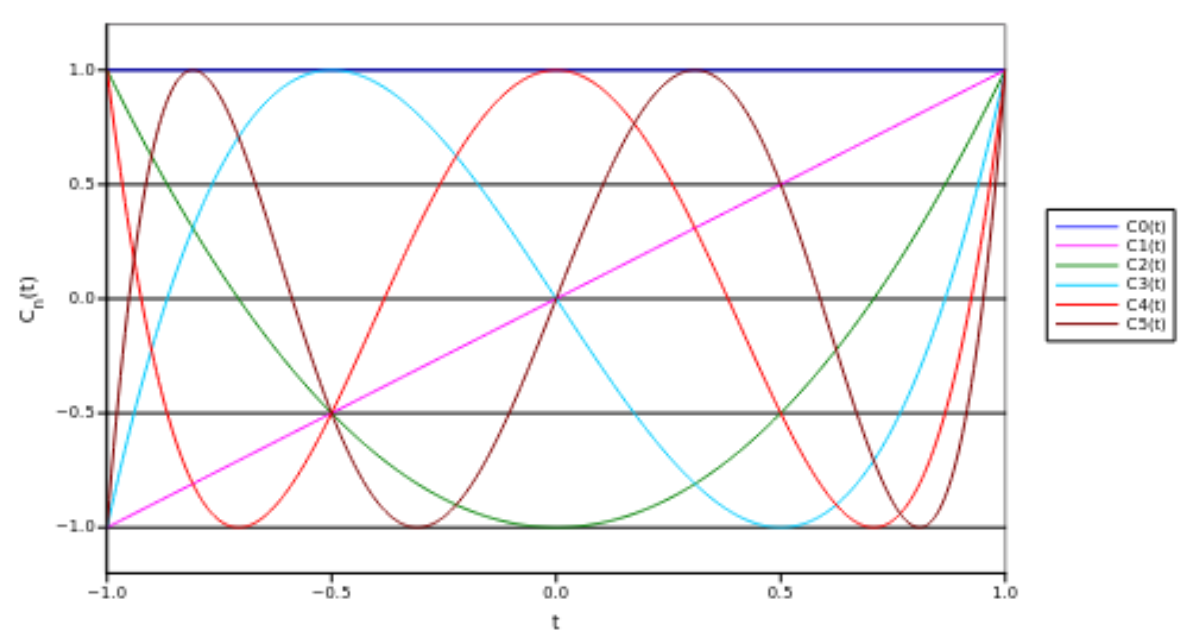
\includegraphics[width=10cm]{img/chebyshev1.png}
	\label{}
	\caption{}
\end{figure}

%
%
\subsection{Implementazione Iterativa}
Grazie alle relazioni di ricorrenza, non è necessario calcolare il polinomio matriciale $P_n\left(\frac{\mathbf{K}}{k^*}\right)$ per tutti i valori di n come richiesto dall'qquazione dei polinomi, ma si può procedere iterativamente:

\[\phi^{(n^* + i + 1)}\ =\ \phi^{(n^* + i)}\, +\, \alpha_n \left(\frac{\mathbf{K}}{k^*} \phi^{(n^* + i)} - \phi^{(n^* + i)}\right)\, +\, \beta_n \left(\phi^{(n^* + i)} - \phi^{(n^* + i - 1)}\right)\ \ ,\]

dove:

\[\alpha_0 = \frac{2}{2 - \sigma}; \quad \alpha_1 = \frac{2}{2 - \sigma - \sigma^2 \frac{\alpha_0}{4}}; \quad \alpha_n = \frac{2}{2 - \sigma - \sigma^2 \frac{\alpha_{n-1}}{8}};
\quad \beta_n = \left(1 - \frac{\sigma}{2}\right) \alpha_n - 1\ .\]

Come si vede in figura, l'accelerazione del metodo di Cebhyshev è molto funzionale per smorzare le armoniche più basse. Per armoniche di ordini superiori può risultare invece meno efficiente del metodo delle potenze stesso.

Nonostante questo, le $n^*$ iterazioni del metodo delle potenze, applicato per ottenere una buona stima, $k^*$, dell'autovalore fondamentale, sono in genere sufficienti a sopprimere tutte le armoniche di ordine superiore al secondo.

\begin{figure}[H]
	\centering
	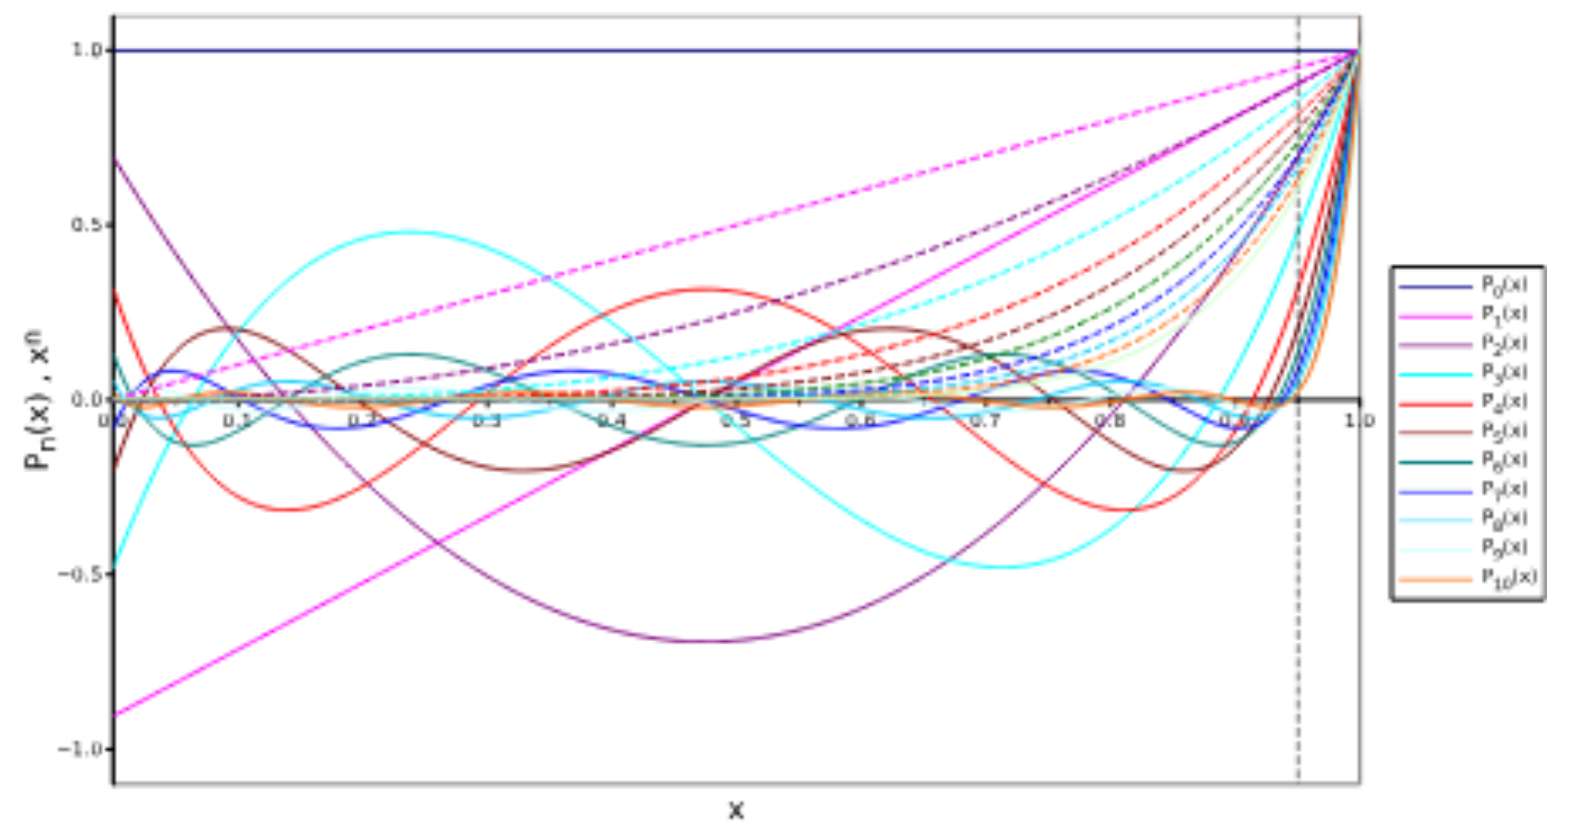
\includegraphics[width=10cm]{img/chebyshev2.png}
	\label{}
	\caption{}
\end{figure}

%
%
\subsection{Confronti e Stima del Dominance Ratio}

Per applicare il metodo di accelerazione di Chebyshev, è necessario avere una stima del dominance ratio $\sigma$. Supponiamo che, dopo $n^*$ iterazioni con il metodo delle potenze, il vettore $\phi^{(n^*)}$ sia approssimato da:

\[\phi^{(n^*)}\ =\ c_1 \varphi_1 + c_2 \varphi_2\ \ .\]

Introducendo il vettore:

\[\delta^{(n)}\ =\ \phi^{(n)} - \phi^{(n-1)}\ \ ,\]

si ha:

\[\begin{aligned}
	\delta^{(n^* + 1)}\ &=\ \phi^{(n^* + 1)} - \phi^{(n^*)}\ =\ \frac{\mathbf{K}}{k^*} \phi^{(n^*)} - \phi^{(n^*)}\ =\\ 
	&=\ \frac{\mathbf{K}}{k^*}\, \left[c_1 \varphi_1 \,+\, c_2 \varphi_2\right] \,-\, c_1 \varphi_1\, -\, c_2 \varphi_2\ =\\
	&= \cancel{c_1 \frac{k_1}{k^*} \varphi_1}\, +\, c_2 \frac{k_2}{k^*} \varphi_2\, -\, \cancel{c_1 \varphi_1}\, -\, c_2 \varphi_2 \ =\ \approx c_2\, (\sigma - 1)\, \varphi_2\ \ .
\end{aligned}\]

Analogamente:

\[\begin{aligned}
	\delta^{(n^* + 2)}\ 
	&=\ \phi^{(n^* + 2)}\, -\, \phi^{(n^* + 1)}\ =\ \left(\frac{\mathbf{K}}{k^*}\right)^2 \phi^{(n^*)}\, -\, \frac{\mathbf{K}}{k^*} \phi^{(n^*)}\ =\\
	&=\ \left(\frac{\mathbf{K}}{k^*}\right)^2\,\left[c_1 \varphi_1 + c_2 \varphi_2\right]\,-\,  \frac{\mathbf{K}}{k^*}\, \left[c_1 \varphi_1 + c_2 \varphi_2\right]\ =\\
	&\approx\ c_2\, \sigma\, (\sigma - 1)\, \varphi_2 
\end{aligned}\]

La stima del dominance ratio si ottiene quindi come:

\[\boxed{\frac{\delta^{(n^* + 2)}}{\delta^{(n^* + 1)}} \approx |\sigma|}\qquad .\]